\section{Introduction}\label{sec:intro}

Getting a quicker validation of the proposed product is crucial in the era of fierce competition and faster obsolescence. Digital product development, which includes, modeling by CAD (Comouter-aided Design)  and analysis by CAE (Computer-aided Engineering) plays a crucial role in quicker ``Time to market''.  For thin-walled models such as sheet-metal/plastic products, a quicker and fairly accurate CAE analysis is possible by idealizing them to their equivalent surface representations, called ``Midsurface''. Midsurface can be envisaged as a surface lying midway of a thin-walled solid, mimicking its shape.   In CAE analysis, instead of using expensive 3D solid elements, 2D surface elements are used on the midsurface for fairly accurate results in lesser computations/time.  Even in the age of scalable and near-infinite computing power, it is still desirable to have  a robust, well-connected midsurface, so as to be able to run more design iterations, quickly.  Because of such advantages, the midsurface functionality is widely used and is available in many commercial CAD-CAE packages. 

\begin{minipage}[h]{\linewidth} 
\begin{minipage}[h]{0.5\linewidth} 
		\centering
		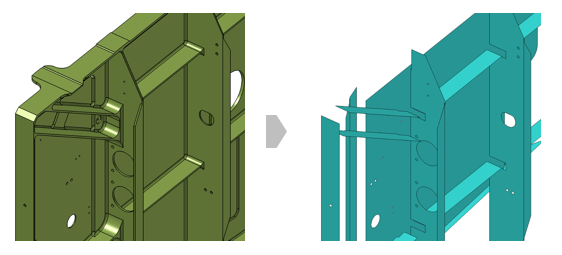
\includegraphics[width=0.9\linewidth]{images/MidsurfaceErrorsMscApex}
		\captionof{figure}{Midsurface Errors (Source: \cite{MScApex})}
		\label{fig:midsurfaceerrors}
\end{minipage}
\hfill
\begin{minipage}[h]{0.5\linewidth} 
In spite of its demand and popularity, the existing techniques of computing the midsurface fail to compute a well-connected midsurface, especially for non-trivial shapes (\cite{Woo2013,Automex}). Failures manifest in the form of gaps, missing patches, overlapping surfaces, not lying midway, not mimicking the input shape, etc. (Figure \ref{fig:midsurfaceerrors}). Correcting these errors is mostly a manual, tedious and highly time-consuming task, requiring hours to days. This correction time can be nearly equivalent to the time it can take to create the midsurface manually from scratch (\cite{Stolt2006}). 
\end{minipage}
\end{minipage}
%\end{figure}



 Automated and  robust technique for computing midsurface  is a crucial need and this work is a step in that direction. Simplification, abstraction and decomposition are the core themes of the proposed approach.

